\documentclass[11pt]{article}
\usepackage[margin=2.2cm]{geometry}
\usepackage{graphicx,booktabs,caption,float,amsmath}
\captionsetup{font=small}
\title{CS6600 Assignment 1: Cache and Memory Hierarchy Simulator}
\author{Shubham Jadhav (CS24S009)}
\date{}
\begin{document}
\maketitle

\section{Simulator and validation}
The simulator (\texttt{cache\_sim.cpp}) is a single generic \texttt{Cache} class that is instantiated as L1 and, optionally, L2. Each set is kept in MRU$\to$LRU order. L1 owns an optional fully associative victim cache (VC). Writes are write-back/write-allocate. A miss on a full L1 set first searches the VC (a \emph{swap request}), and a hit swaps the two blocks. On a VC miss the L1 victim enters the VC, a dirty block pushed out of the VC is written back, and the missing block is read from the next level. L2 is non-inclusive. CACTI supplies hit time, energy and area (a VC that CACTI cannot model uses $HT_{VC}=0.2$~ns).

All 8 reference outputs match with \texttt{diff -iw}: raw statistics, the contents of L1, VC and L2 in MRU$\to$LRU order, AAT, EDP and area, with EDP matching digit for digit. A further 20 outputs (L1 from 8~KB to 1~MB, associativity up to 512, block sizes up to 2~KB, VC with 4--14 blocks, L2 up to 8~MB) also match for every line they contain. All experiments below use the provided \texttt{gcc} trace and are produced by \texttt{run\_experiments.py}.

\paragraph{CACTI limits.} CACTI cannot model some very small or highly associative arrays (for example a 1~KB or 2~KB 4-way cache, a 2~KB 8-way cache or a 512~KB 2-way cache with 32~B blocks). For those configurations AAT, EDP and area are undefined, so they appear as gaps in the plots; miss rates are unaffected.

\section{L1 size and associativity}
\begin{figure}[H]\centering
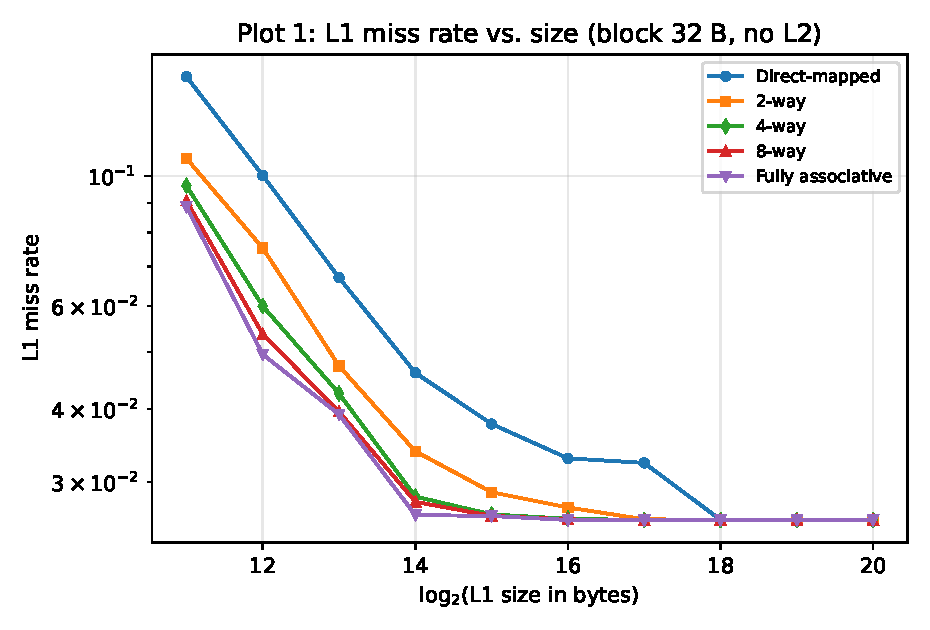
\includegraphics[width=.49\linewidth]{plots/plot1_missrate.pdf}\hfill
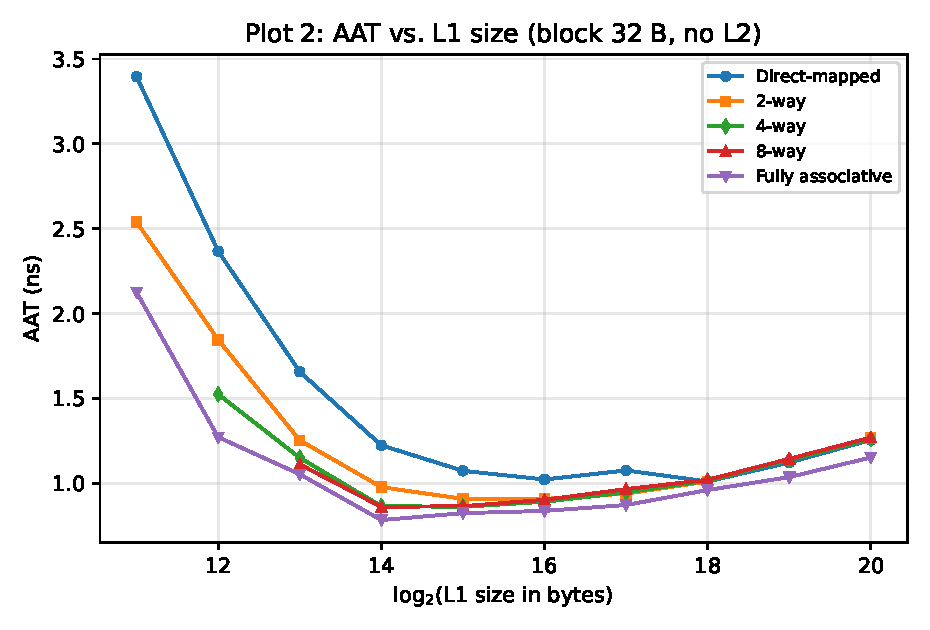
\includegraphics[width=.49\linewidth]{plots/plot2_aat.pdf}
\caption{Plot 1 (L1 miss rate, log scale) and Plot 2 (AAT) versus L1 size for block size 32~B and no L2.}
\end{figure}

\paragraph{Plot 1: trends.} Miss rate falls steadily with size and with associativity and then flattens. A direct-mapped cache falls from 14.8\% at 2~KB to 3.2\% at 128~KB. 4-way and 8-way caches reach the floor near 32~KB (2.64\% and 2.62\%), and every curve reaches 2.58\% by 256~KB. Associativity helps most for small caches: at 2~KB, going from direct-mapped to 8-way cuts the miss rate by about 40\% (14.8\% to 9.1\%), whereas at 128~KB the 2-way, 4-way and 8-way caches are indistinguishable.

\paragraph{Compulsory miss rate.} The floor is the miss rate of a cache large enough to hold the whole footprint: 2.58\% (identical at 256~KB and 1~MB, fully associative).

\paragraph{Conflict miss rate} (miss rate of the A-way cache minus that of the fully associative cache of the same size, in percentage points):
\begin{center}\small
\begin{tabular}{lrrrrrrr}\toprule
Size & 2 KB & 4 KB & 8 KB & 16 KB & 32 KB & 64 KB & 128 KB\\\midrule
Direct-mapped & 5.91 & 5.06 & 2.79 & 1.98 & 1.14 & 0.71 & 0.65\\
2-way & 1.85 & 2.57 & 0.82 & 0.75 & 0.26 & 0.13 & 0.01\\
4-way & 0.76 & 1.04 & 0.33 & 0.20 & 0.02 & 0.01 & 0.00\\
8-way & 0.21 & 0.41 & 0.04 & 0.14 & 0.00 & 0.01 & 0.00\\\bottomrule
\end{tabular}\end{center}
The remaining part of the fully associative miss rate above 2.58\% is the capacity miss rate (6.3 points at 2~KB, 2.4 at 4~KB, 1.3 at 8~KB, nearly 0 from 16~KB). A direct-mapped cache still has 0.65 points of conflict misses at 128~KB, so conflicts outlive capacity misses.

\paragraph{Plot 2: best AAT without L2.} Hit time rises with size and associativity, so AAT has an interior minimum: 4-way and 8-way curves bottom out at 0.86~ns (16--32~KB) and rise again to 1.27~ns at 1~MB, where the miss rate is already at its floor. The lowest AAT of all is the \textbf{16~KB fully associative} cache at 0.784~ns (the CACTI model of a small CAM is fast), with EDP $4.6\times10^{8}$ and area 0.063~mm$^2$. The best set-associative choices are 16~KB 8-way and 32~KB 4-way, both at 0.862~ns; the 16~KB 8-way point has EDP $1.46\times10^{8}$ and area 0.121~mm$^2$.

\section{Adding an L2}
\begin{figure}[H]\centering
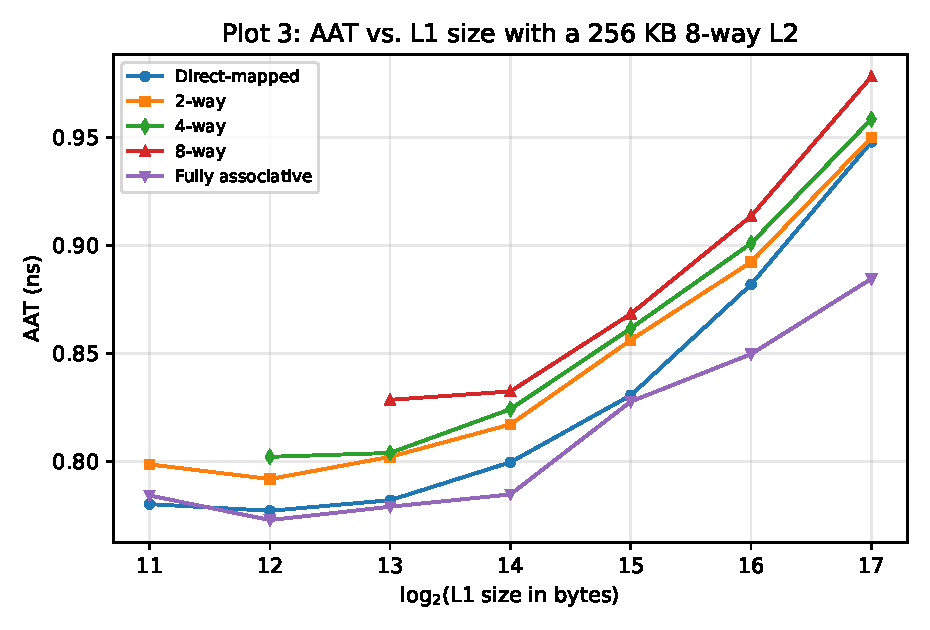
\includegraphics[width=.5\linewidth]{plots/plot3_aat_l2.pdf}
\caption{Plot 3: AAT versus L1 size with a 256~KB 8-way L2.}
\end{figure}
With the L2 the miss penalty seen by L1 collapses from about 22~ns to $HT_{L2}+MR_{L2}\times 22$~ns, so a cheap, fast L1 wins and the best L1 shrinks to 4~KB. The best AAT is \textbf{0.773~ns with a 4~KB fully associative L1} (0.777~ns for the 4~KB direct-mapped L1; 0.779~ns for 8~KB fully associative). Compared with the best L1-only AAT this is a 1.5\% improvement over 0.784~ns (fully associative) and a 9.9\% improvement over 0.862~ns when only set-associative L1 caches are allowed (0.777~ns, 4~KB direct-mapped).

\emph{EDP and area.} With the 4~KB direct-mapped L1 + L2 the EDP is $6.8\times10^{7}$ versus $1.46\times10^{8}$ for the best L1-only set-associative design (about 2.2$\times$ better), and it is about 7$\times$ better than the fully associative L1-only design ($4.6\times10^{8}$). The price is area: 1.20~mm$^2$ versus 0.12~mm$^2$ (about 10$\times$) because the 256~KB L2 dominates. The L2 buys energy by filtering DRAM traffic and costs silicon.

\section{L1 size and block size}
\begin{figure}[H]\centering
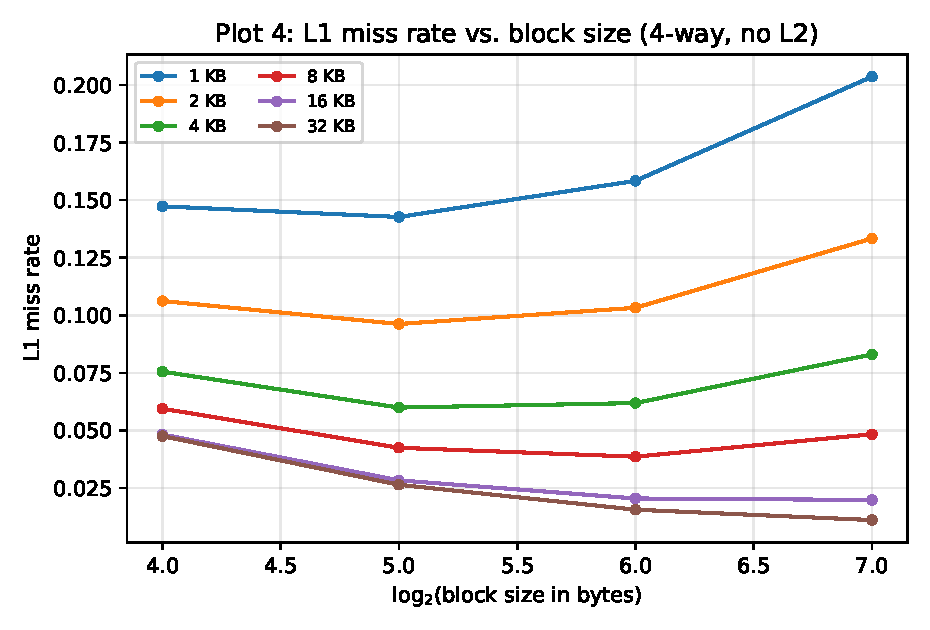
\includegraphics[width=.5\linewidth]{plots/plot4_blocksize.pdf}
\caption{Plot 4: L1 miss rate versus block size for a 4-way L1, no L2.}
\end{figure}
The spatial-locality versus pollution trade-off is clear and depends on cache size. For 1--4~KB caches the miss rate is lowest at 32~B and rises sharply for 128~B (1~KB: 14.3\% at 32~B, 20.4\% at 128~B), because few large blocks mean few distinct blocks: pollution and conflicts dominate. For an 8~KB cache the minimum moves to 64~B (3.86\%, versus 4.25\% at 32~B and 4.83\% at 128~B). For 16~KB and 32~KB caches larger blocks keep helping (32~KB: 4.75, 2.64, 1.56, 1.11\% for 16, 32, 64, 128~B). The \textbf{optimal block size for an 8~KB 4-way L1 is 64~B} by miss rate; by AAT also 64~B (1.139~ns versus 1.151~ns at 32~B). A 16~B block is never best: its miss rate is highest for $\ge$8~KB caches.

\section{L1 + L2 co-optimisation}
\begin{figure}[H]\centering
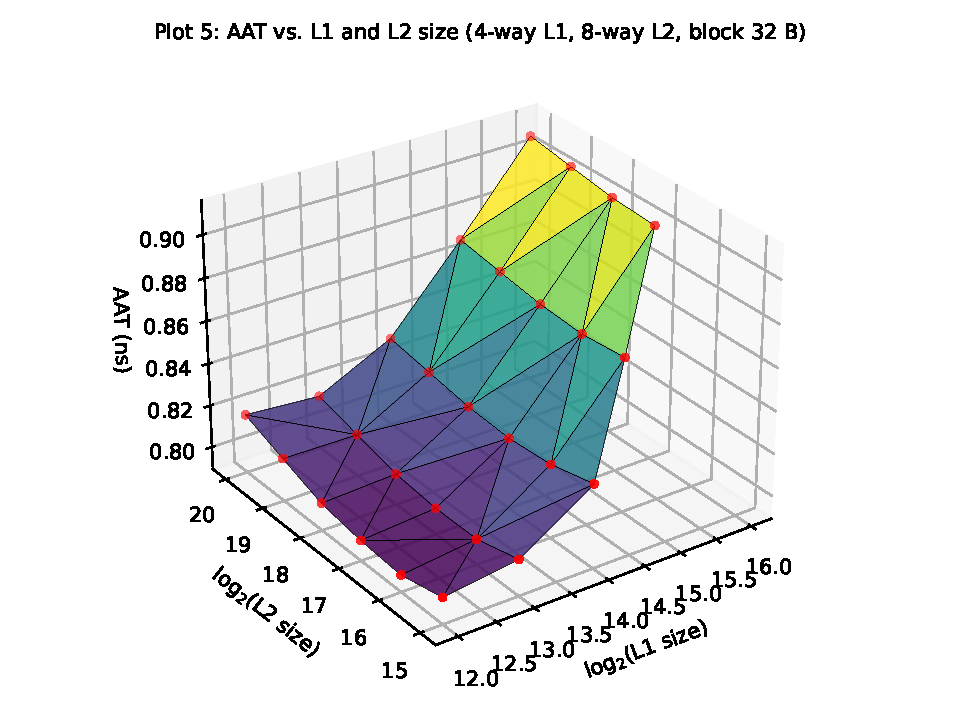
\includegraphics[width=.49\linewidth]{plots/plot5_aat_surface.pdf}\hfill
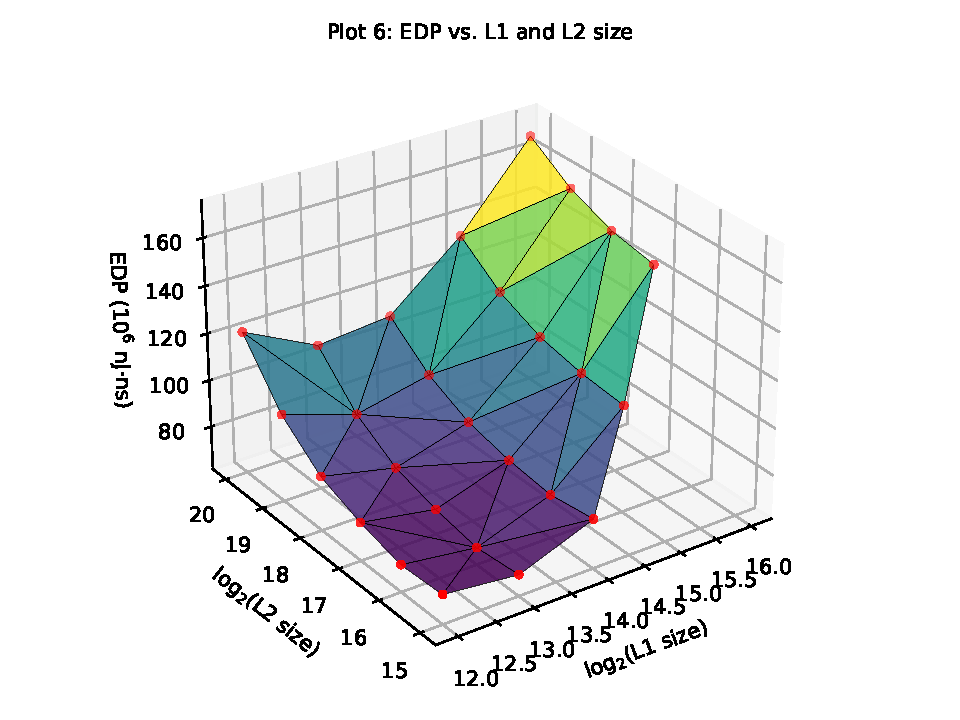
\includegraphics[width=.49\linewidth]{plots/plot6_edp_surface.pdf}
\caption{Plot 5 (AAT) and Plot 6 (EDP) for a 4-way L1 and 8-way L2, block 32~B, only points with L1 smaller than L2. CACTI cannot model a 1~KB or 2~KB 4-way L1 (and the 32~KB L1 with a 32~KB L2 is excluded), so those points are missing.}
\end{figure}
\paragraph{Best AAT.} The best AAT is \textbf{0.797~ns with a 4~KB L1 and a 64~KB L2} (area 0.386~mm$^2$). The surface is almost flat in L2 size (0.797--0.82~ns for the 4~KB L1) and rises with L1 size, because the L1 hit time is paid on every access while a bigger L2 only helps the few L1 misses.

\paragraph{Smaller design within 5\%.} A 4~KB L1 with a \textbf{32~KB L2} has AAT 0.802~ns (0.6\% above the best) with area 0.285~mm$^2$, 26\% smaller; an 8~KB L1 with a 32~KB L2 (0.806~ns, +1.1\%, 0.309~mm$^2$) also qualifies.

\paragraph{Best EDP (Plot 6).} The best EDP is \textbf{$6.86\times10^{7}$ with an 8~KB L1 and a 64~KB L2} (AAT 0.801~ns, area 0.410~mm$^2$). EDP grows quickly with L2 size because the energy of every L2 access grows with its size, so energy favours small L2s even more than AAT does.

\section{Victim cache}
\begin{figure}[H]\centering
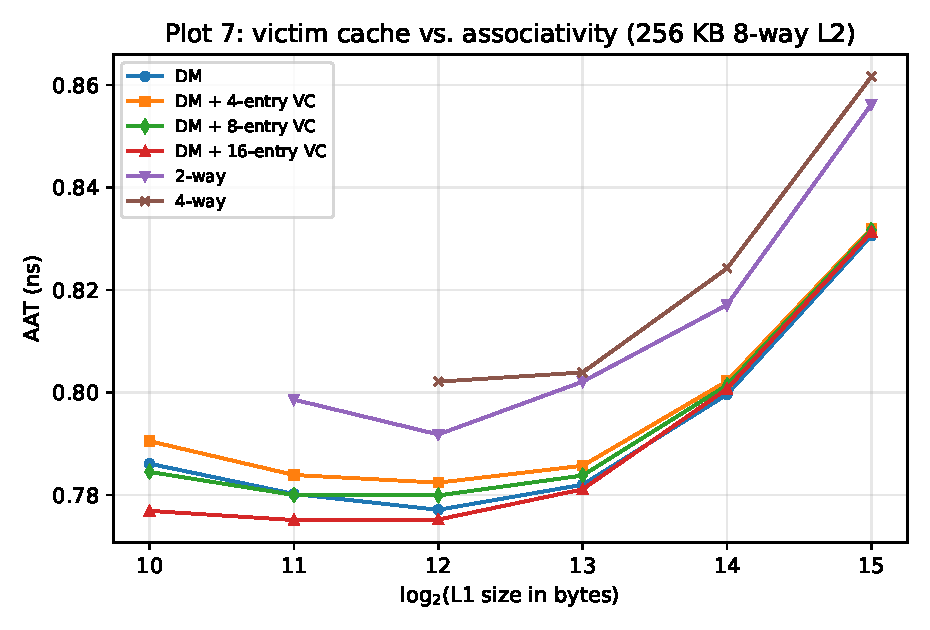
\includegraphics[width=.5\linewidth]{plots/plot7_victim.pdf}
\caption{Plot 7: AAT versus L1 size with a 256~KB 8-way L2. Missing points are CACTI failures for the 1~KB and 2~KB 4-way cache and the 1~KB 2-way cache.}
\end{figure}
\paragraph{VC versus 2-way.} For small direct-mapped caches a victim cache does better than doubling the associativity: at 2~KB a direct-mapped L1 with a 16-entry VC has AAT 0.775~ns against 0.780~ns for direct-mapped and 0.799~ns for 2-way; at 4~KB it is 0.775 versus 0.777 and 0.792. The 2-way cache removes the same conflicts but pays a longer hit time on every access, while the VC is probed only on a miss in a full set (swap request rate 0.15 at 2~KB, 0.10 at 4~KB and 0.03 at 32~KB). For 8~KB and larger the VC gains vanish (16~KB: 0.8007 with a 16-entry VC versus 0.7996 without; 32~KB: 0.8313 versus 0.8306 for direct-mapped), because the conflict misses it catches are few and the extra swap-request time and energy outweigh them.

\paragraph{Best configuration.} Among the Plot~7 configurations the best AAT is \textbf{a direct-mapped L1 of 2~KB or 4~KB with a 16-entry VC, 0.775~ns} (0.7751 and 0.7752~ns). Smaller VCs help less (4 and 8 entries give 0.784 and 0.780~ns for the 2~KB cache).

\paragraph{Smaller area within 5\%.} Almost all of the area is the 256~KB L2 (1.2~mm$^2$). Replacing it by a 32~KB 8-way L2 gives a \textbf{4~KB direct-mapped L1 + 16-entry VC + 32~KB L2} with AAT 0.774~ns (slightly \emph{better}) and area 0.285~mm$^2$ (76\% smaller); with a 2~KB L1 the AAT is 0.770~ns at 0.264~mm$^2$.

\end{document}
